\newcounter{qt}

\begin{frame}
  \begin{enumerate}
    \item Indítsuk el a Qt Creatort.\\
      \resizebox{0.4\textheight}{!}{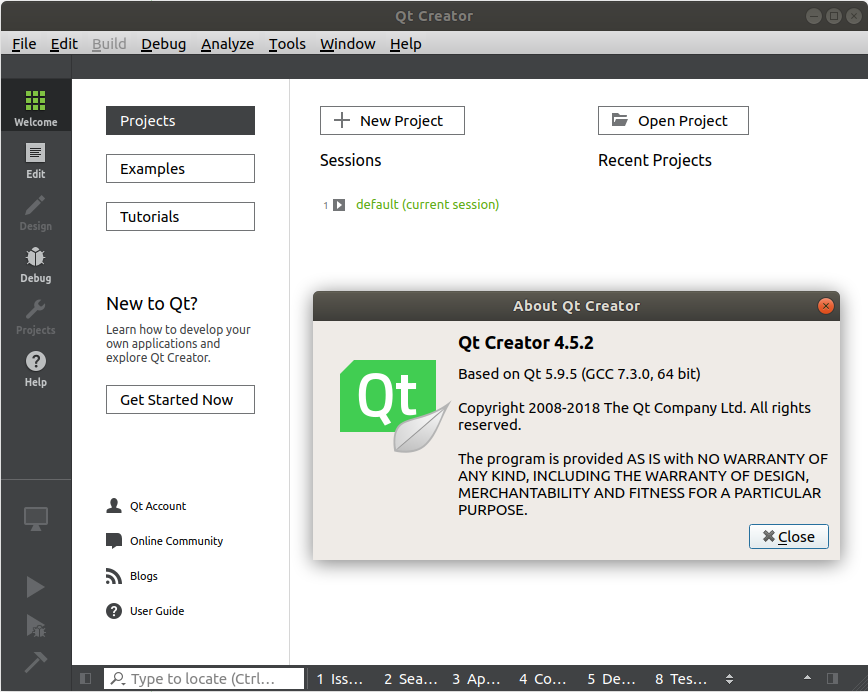
\includegraphics{./qtcreator.png}}
    \item Készítsünk új projektet az osztályunk működésének kipróbálásához (egyelőre googletest nélkül)! \emph{File $\to$ New File or Project...}
    \item A dialógusablakban jelöljük meg a \emph{Non-Qt Project}-et majd a \emph{Plain C++ Application}-t! Végül kattintsunk a \emph{Choose...} gombra!\\
      \resizebox{0.4\textheight}{!}{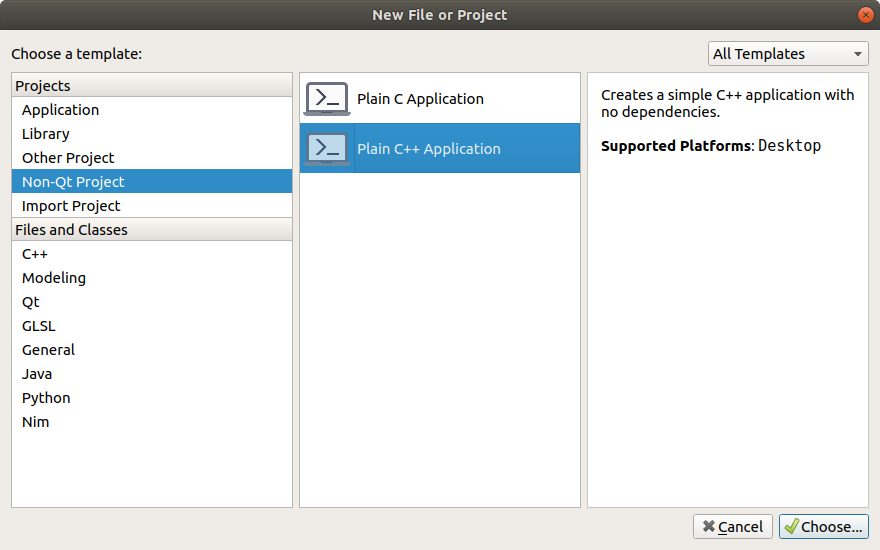
\includegraphics{./newFileOrProject.png}}
    \setcounter{qt}{\theenumi}
  \end{enumerate}
\end{frame}

\begin{frame}
  \begin{enumerate}
    \setcounter{enumi}{\theqt}
    \item A dialógusablakban adjuk meg a projekt nevét a \emph{Name} mezőben (\texttt{szematrix}), és válasszunk egy mappát, ahová a projektet elhelyezhetjük! Végül lépjünk a következő oldalra (\emph{Next})!\\
      \resizebox{0.4\textheight}{!}{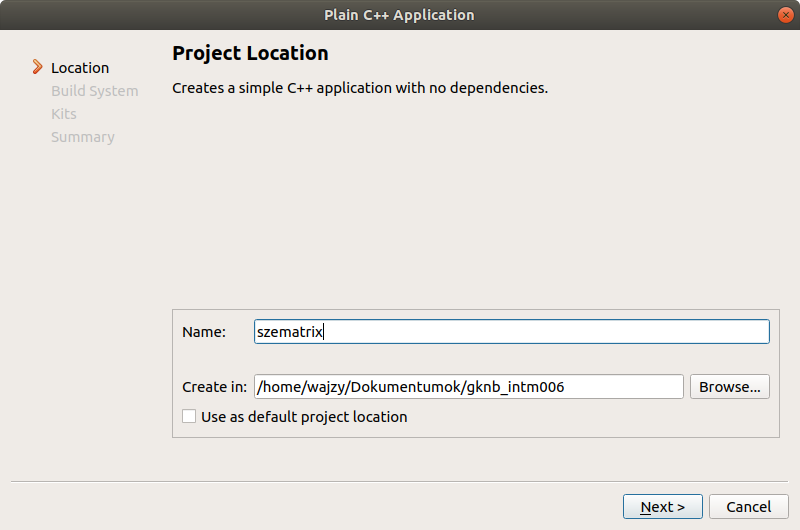
\includegraphics{./plainCppApplication1.png}}
    \item Az építő rendszer elvileg lehetne \emph{cmake} is, de ezt az IDE nem támogatja teljeskörűen, ezért őrizzük meg az alapértelmezett \emph{qmake}-et, majd lépjünk a következő oldalra!\\
      \resizebox{0.4\textheight}{!}{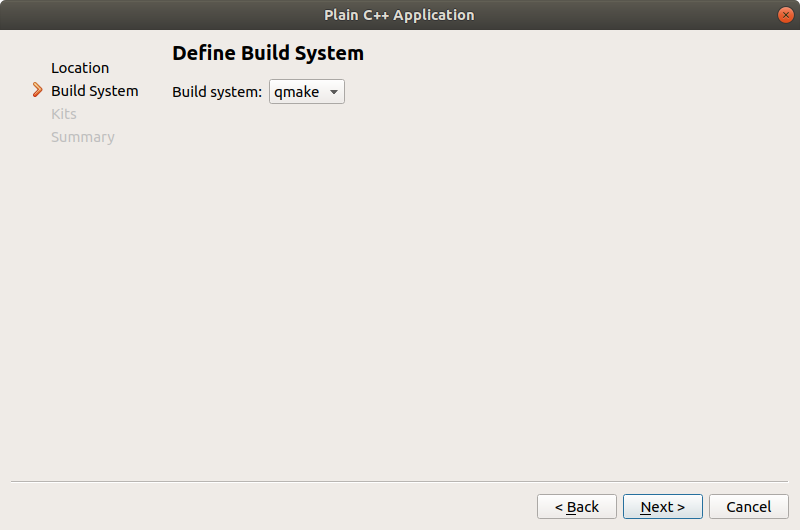
\includegraphics{./plainCppApplication2.png}}
    \setcounter{qt}{\theenumi}
  \end{enumerate}
\end{frame}

\begin{frame}
  \begin{enumerate}
    \setcounter{enumi}{\theqt}
    \item A készleteknél (\emph{Kit Selection}) hagyjunk mindent változatlanul!
    \item A következő oldalon, az \emph{Add to version control...}-nál lehetne beállítani a Git verziókezelőt, de mivel nincs hosszabb távú célunk a projekttel, nem élünk a lehetőséggel.\\
    A dialógusablak alján látszik, hogy létrejön a \emph{qmake} projektleíró fájlja (\texttt{szematrix.pro}) illetve egy helykitöltő forrásszöveg (\texttt{main.cpp}), amit hamarosan lecserélünk.\\
      \resizebox{0.4\textheight}{!}{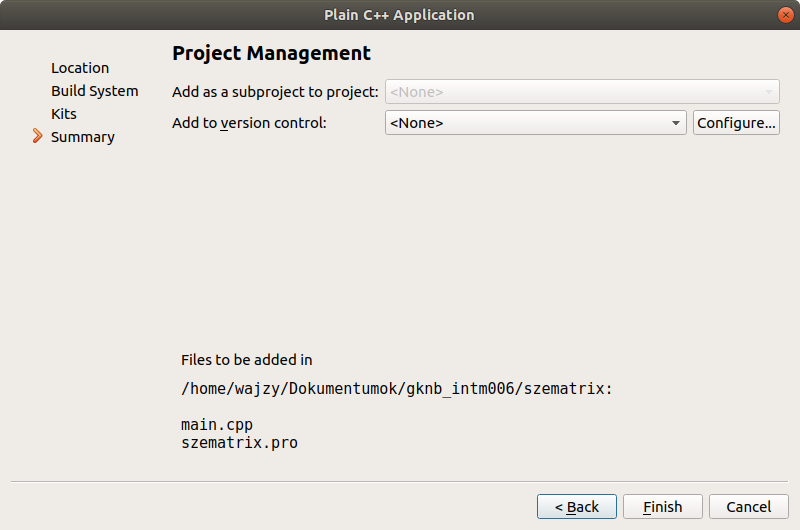
\includegraphics{./plainCppApplication4.png}}
    \setcounter{qt}{\theenumi}
  \end{enumerate}
\end{frame}

\begin{frame}
  \begin{enumerate}
    \setcounter{enumi}{\theqt}
    \item Másoljuk a projekt mappájába a \texttt{01/example01.cpp} és \texttt{14/matrix14.h} fájlokat!
    \item A \emph{Projects} nézetben kattintsunk jobb gombbal a projekt nevén (\emph{szematrix}), a kinyíló menüben pedig válasszuk az \emph{Add Existing Files...} pontot! Adjuk hozzá a projekthez az előbb bemásolt két állományt!
    \item Kattintsunk jobb gombbal a \emph{main.cpp}-n, majd válasszuk a \emph{Remove File...} lehetőséget, azaz töröljük a generált állományt! Ne sajnáljuk a fájlt véglegesen törölni (\emph{Delete file permanently}).
    \item Nyissuk meg az \texttt{example01.cpp} fájlt a nevére duplán kattintva, majd módosítsuk a második sort, hogy a \texttt{matrix14.h}-ra hivatkozzon!
    \setcounter{qt}{\theenumi}
  \end{enumerate}
\end{frame}

\begin{frame}
  \begin{enumerate}
    \setcounter{enumi}{\theqt}
    \item Ezután a program fordítható, futtatható (\emph{Build} $\to$ \emph{Run}, vagy a zöld háromszögre kattintva).\\
    \resizebox{\textheight}{!}{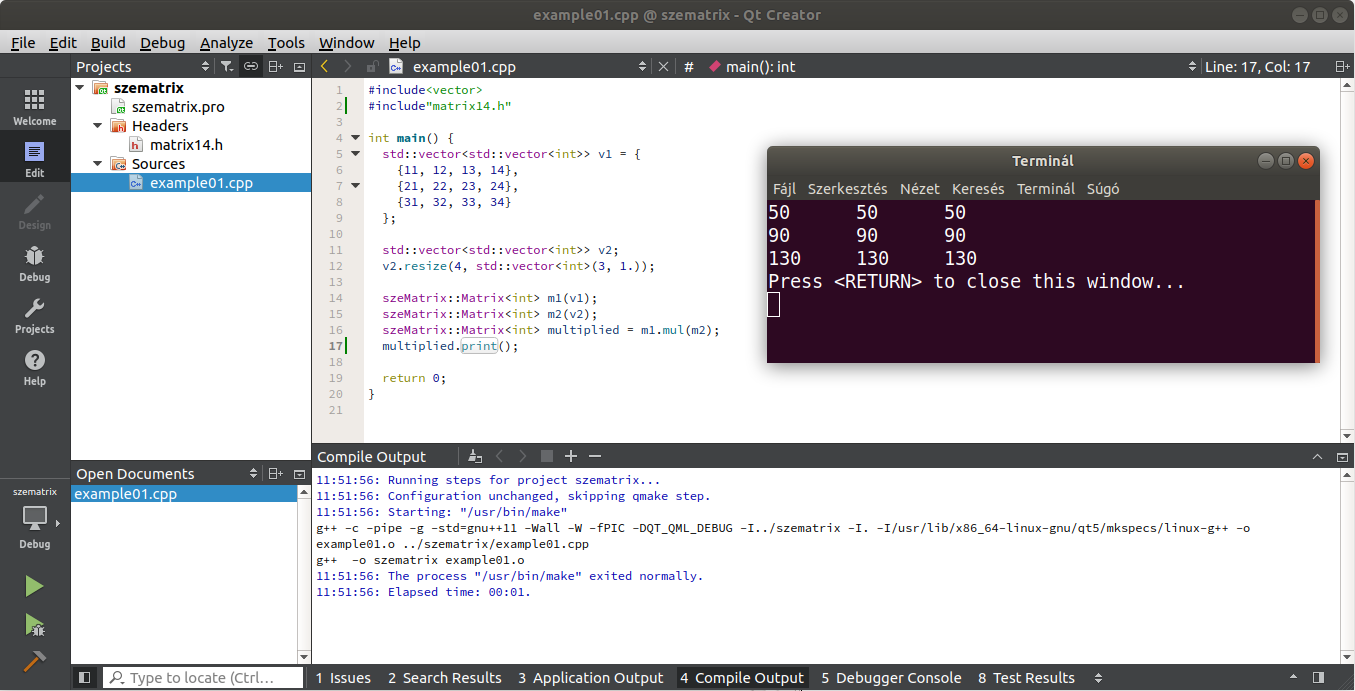
\includegraphics{./szematrix.png}}
    \setcounter{qt}{\theenumi}
  \end{enumerate}
\end{frame}

\begin{frame}
  \begin{enumerate}
    \setcounter{enumi}{\theqt}
    \item Készítsük el a teszt projektet! A \emph{File $\to$ New File or Project...} menüvel megnyíló ablakban most válasszuk az \emph{Other Project}-et, majd az \emph{Auto Test Project}-et!\\
    \item A megnyíló dialógusablak \emph{Name} mezőjébe gépeljük az új projekt nevét: \texttt{matrixteszt}!
    \item A következő fülön kell kiválasztani a tesztelés eszközét, ami legyen \emph{Googletest}! Bár most erre semmi szükségünk, kénytelenek vagyunk megadni egy helykitöltő teszteset-nevet (\emph{Test case name}, pl. \texttt{case1}) és tesztkészlet-nevet (\emph{Test set name}, pl. \texttt{set1}). Engedélyezzük a C++11-kompatibilis fordítást a jelölőnégyzettel, majd adjuk meg a \emph{googletest} könyvtárát! Most is őrizzük meg a \emph{qmake} építő rendszert!\\
    \resizebox{\textheight}{!}{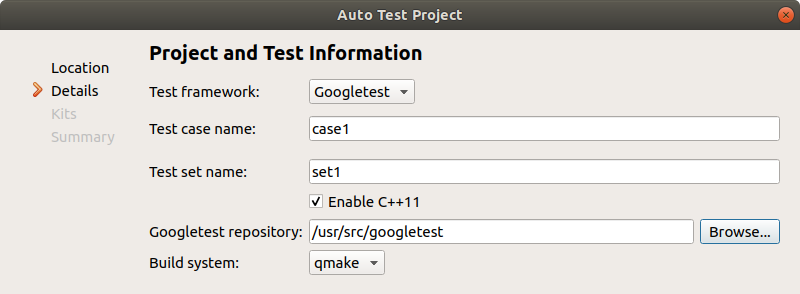
\includegraphics{./autoTestProject.png}}
    \setcounter{qt}{\theenumi}
  \end{enumerate}
\end{frame}

\begin{frame}
  \begin{enumerate}
    \setcounter{enumi}{\theqt}
    \item A \emph{Next}, majd \emph{Finish} gombokra kattintva létrejön, és aktívvá válik a teszt projekt.
    \item A projekt mappájába (\texttt{matrixteszt}) másoljuk be a \texttt{14/matrix14test.cpp} fájlt! A \emph{Projects} nézetben a projekten jobb gombbal kattintva válasszuk az \emph{Add Existing Files...} pontot, és adjuk hozzá az átmásolt fájlt a projekthez!
    \item Nyissuk meg a fájlt a szerkesztőben, majd módosítsuk az első sort: \texttt{\#include"../szematrix/matrix14.h"}
    \item Távolítsuk el a projektből a \texttt{main.cpp} és \texttt{tst\_case1.h} fájlokat (Del gomb)!
    \item A tesztprogram a zöld gombbal fordítható, futtatható.
    \setcounter{qt}{\theenumi}
  \end{enumerate}
\end{frame}

\begin{frame}
  \begin{itemize}
    \item Futtatandó tesztesetek kiválasztása: \emph{Tests} nézetben.\\
      \resizebox{0.5\textheight}{!}{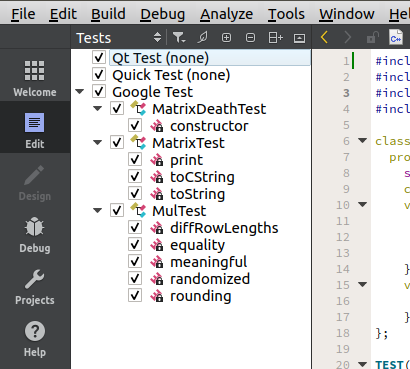
\includegraphics{./tests.png}}
    \item Kiválasztott/összes teszteset futtatása: \emph{Test Results} kimeneti ablaktábla (\emph{Window $\to$ Output Panes $\to$ Test Results}) zöld háromszögeivel\\
      \resizebox{0.5\textheight}{!}{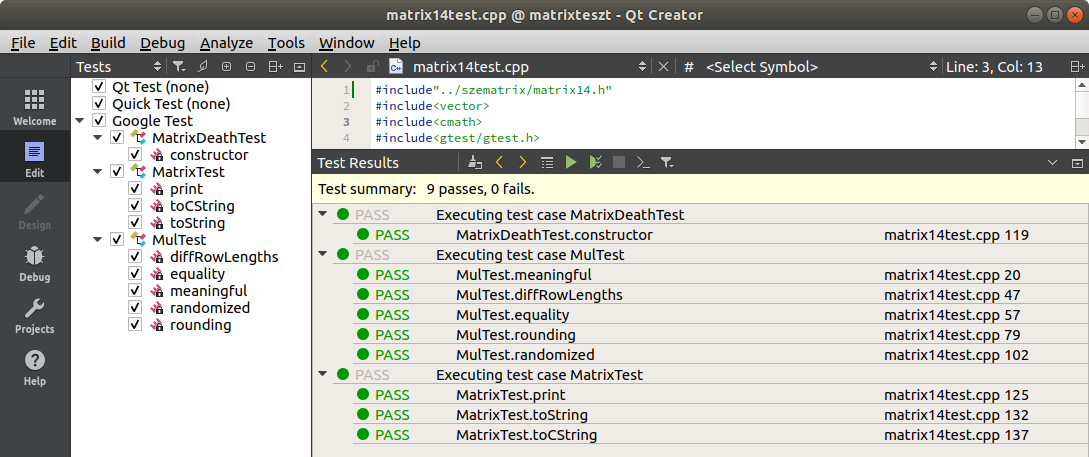
\includegraphics{./outputPane.png}}
  \end{itemize}
\end{frame}

\begin{frame}
  \begin{itemize}
    \item További beállítások: \emph{Tools $\to$ Options... $\to$ Testing}\\
      \resizebox{\textheight}{!}{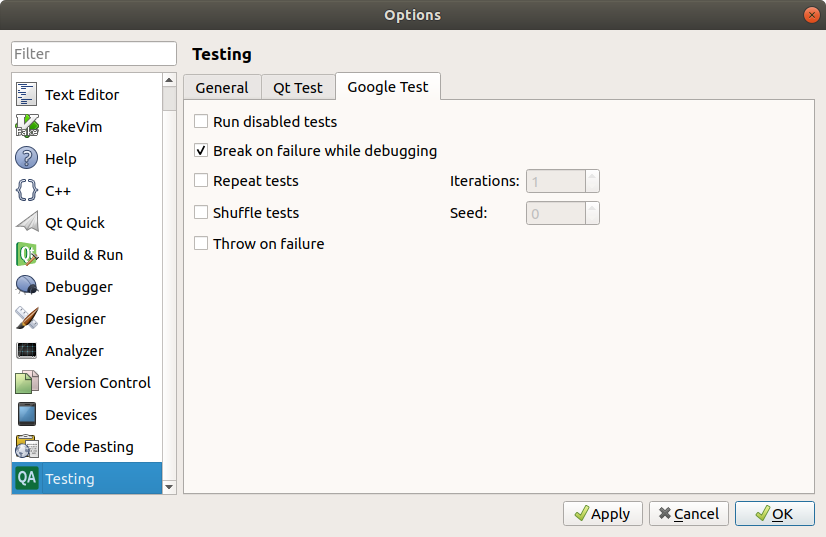
\includegraphics{./options.png}}
  \end{itemize}
\end{frame}
